

%%%%%%%%%%%%%%%%%%%%%%% file template.tex %%%%%%%%%%%%%%%%%%%%%%%%%
%
% This is a template file for the global option of the SVJour class
%
% Copy it to a new file with a new name and use it as the basis
% for your article
%
%%%%%%%%%%%%%%%%%%%%%%%% Springer-Verlag %%%%%%%%%%%%%%%%%%%%%%%%%%
%
% First comes an example EPS file -- just ignore it and
% proceed on the \documentclass line
%\begin{filecontents*}{example.eps}
%%!PS-Adobe-3.0 EPSF-3.0
%%%BoundingBox: 19 19 221 221
%%%CreationDate: Mon Sep 29 1997
%%%Creator: programmed by hand (JK)
%%%EndComments
%gsave
%newpath
%  20 20 moveto
%  20 220 lineto
%  220 220 lineto
%  220 20 lineto
%closepath
%2 setlinewidth
%gsave
%  .4 setgray fill
%grestore
%stroke
%grestore
%\end{filecontents*}
%
% Choose either the first of the next two \documentclass lines for one
% column journals or the second for two column journals.
% Make sure that meanwhile no specific package for your very project has
% appeared by viewing the web page
% http://www.springer.de/author/tex/help-journals.html
\documentclass[global]{svjour}
%\documentclass[global,twocolumn,referee]{svjour}
% Remove option referee for final version
%
% Remove any % below to load the required packages
%\usepackage{latexsym}
\usepackage{lscape,amsmath,epsfig}
\usepackage{algorithm}
\usepackage{algorithmic}
\usepackage{amssymb}
\usepackage{array}
\usepackage{graphicx} % for pdf, bitmapped graphics files
\usepackage[tight]{subfigure}
\usepackage{eurosym}
% etc
%
% Insert the name of "your" journal with the command below:
\journalname{Evolutionary Intelligence}
%

\newcounter{linecounter}
\newcommand{\linenumbering}{\makebox[2em][r]{\arabic{linecounter}:}}
\renewcommand{\line}[1]{\refstepcounter{linecounter}
\linenumbering}
\newcommand{\resetline}{\setcounter{linecounter}{0}}


\begin{document}

\title{MasterMind Game: New Solver and Optimal Anticipation Strategies Design based on Evolutionary Computation}

\author{J. Maestro-Montojo$^\dag$, S. Salcedo-Sanz$^\dag$ and J. J. Merelo$^\ddag$}
%% \thanks is optional - remove next line if not needed
%\thanks{\emph{Present address:} Insert the address here if needed}%
%}                     % Do not remove
%%
%\offprints{}          % Insert a name or remove this line
%%
\institute{$^\dag$ Department of Signal Theory and Communications,
Universidad de Alcal\'a, Escuela Polit\'ecnica Superior, 28871
Alcal\'a de Henares, Madrid, Spain. email address:
sancho.salcedo@uah.es\\
$^\ddag$ Departamento de Arquitectura y Tecnolog\'{\i}a de Computadores,
Universidad de Granada,
Granada, Spain.}

%
\date{Received: date / Revised version: date}
% The correct dates will be entered by the editor
%
\authorrunning{Maestro-Montojo et al.}
\titlerunning{New Evolutionary Computation Approaches for MasterMind}
\maketitle
%
\begin{abstract}
This paper presents evolutionary solutions the well-known MasterMind
game, a classic board game invented in the 1970's. First, we propose a
novel evolutionary approach (which we call {\em nested hierarchical evolutionary search}) to solve the MasterMind game, comparing the obtained
results with that of existing algorithms. Second, we show how to design novel game anticipation strategies for the MasterMind game, by
applying  Genetic Programming. In this case we compare the performance of the new obtained strategies with
that of the classical ones, obtaining advantages in all the cases tested.
\end{abstract}
%
\begin{keywords}
MasterMind, Evolutionary algorithms, Genetic Programming, Anticipation strategies.
\end{keywords}

\section{Introduction and state of the art}

MasterMind is a classic board game for two players, invented by
M. Meirowitz in 1970. One of the players acts as a {\em codemaker},
and the other one as {\em codebreaker}. The codemaker starts the game
by choosing a secret code, i.e. a sequence of $P$ different colored pegs, out of $N$ possible colors (repetitions are allowed). The
codebreaker tries to guess the code by means of a set of
guesses. After each guess, the codemaker gives an answer to the guess,
in terms of two numbers: a number of black pegs for those elements in
the guess that coincide in color and position with the ones in the
secret code, and a number of  white pegs for those elements in the
guess that coincide in color, but not in position with the ones of the
secret code. Figure \ref{Game_Mastermind} shows an example of the game,
with the secret code and two guesses (with their respective answers).


\begin{figure}[!ht]
\begin{center}
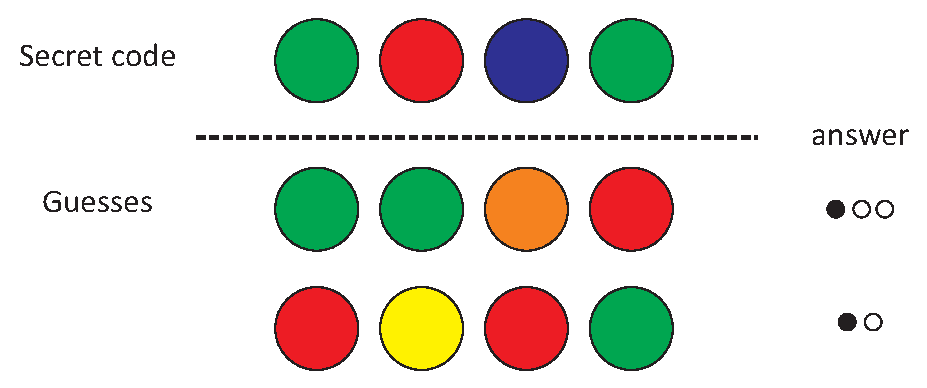
\includegraphics[draft=false,angle=0,width=6cm]{./Ejemplo_juego.eps}
\end{center}
\caption{\label{Game_Mastermind} Example of a MasterMind game.}
\end{figure}

MasterMind is a challenging problem from the algorithmic point of
view. The game caught the attention of many researchers by the end of
the seventies so there are a good amount of works dealing with this
problem in the literature. Different techniques have been applied to
the solution of the problem: full enumeration approaches, heuristics
based on simple rules and also meta-heuristic algorithms.

Among full enumeration techniques, the pioneering proposal by Knuth et
al. \cite{Knuth77} (known as Worst Case strategy) was able to
succeed for $N=4,P=6$ in less than five moves, and was based on choosing the
combination that minimizes the maximum number of remaining eligible
codes. Other approaches to MasterMind applying full enumeration
techniques are \cite{Irving79,Koyoma93}. In \cite{Bestavros86}, a full
enumeration technique was mixed with Information Theory in order to
obtain the best enumeration strategy. This approach was named as ``Max
Entropy'' and is currently in use in different algorithms for the
MasterMind. In \cite{Kooi05} the strategy known as ``Most Parts'' were
introduced and applied to obtain a solid exhaustive algorithm to the
problem. More recently, in \cite{Chen07} and \cite{Chen07b}, a variant
of full enumeration via depth-first search is proposed, and in
\cite{Merelo12} different new exhaustive search strategies are
proposed, after a full statistical revision of the problem and
alternative exhaustive approaches.

In a different approach to the problem, there are different heuristic-based approaches which try to
obtain good solutions to the problem with a short computation
time. The first approach of this kind is \cite{Shapiro83}, where the
codebreaker constructs a list of colors elements, and for each guess,
he starts from the last examined position in the previous guess until
find an eligible code. The approach in \cite{Swaszek00} is similar,
with a variant in the ordering colors in the list. In \cite{Kovacs03}
a hill climbing approach is proposed, which minimizes the average
number of guesses and also the number of evaluated codes. The most
recent approaches to MasterMind relay on meta-heuristics
algorithms. The first evolutionary-based algorithms for tackling the
MasterMind game appeared in the last 90's and first years of 2000
\cite{Bernier96,Bento99,Kalister03}. More recently, in \cite{Merelo06}
a stepwise evolutionary approach was first proposed. That approach
played any eligible code as soon as it was found by the algorithm. A
subsequent approach also based on evolutionary algorithm was presented
in \cite{Berghman09}, where an evolutionary algorithm selects a number
of eligible codes, and then the one played is selected by a mechanism
of Expected Size. The most recent approach to MasterMind with
evolutionary computation was presented in \cite{Maestro13}, where
new strategies to improve the performance of evolutionary algorithms
in MasterMind were suggested. 

In this paper we deal with MasterMind using evolutionary techniques,
by focussing on two different aspects of the game. First, propose a novel evolutionary approach to solve the game
based on a nested hierarchical evolutionary search. The
proposed approach solves the problem by an initial evolutionary search
of the eligible set, and a second evolutionary approach to obtain the
best possible guess to play, based on different predictive
strategies. We present a comparison study of the performance of the
proposed nested hierarchical approach with alternative techniques in the literature.
Second, we propose a new method for designing anticipation strategies for the MasterMind,
based on a Genetic Programming algorithm. We detail the proposed approach and
operators used in the algorithm, and then we test the method by obtaining new anticipation
strategies for the game, in different instances.

The structure of the rest of the paper is the following: next section
presents some important notation and definitions about MasterMind. Section \ref{ss:bs} presents the nested
hierarchical evolutionary algorithm introduced in this paper. Section \ref{GP} presents the
Genetic Programming approach to evolve new anticipation strategies for the game.
Section \ref{Experiments} shows the results obtained by both proposed approaches in a
number of numerical experiments, to show the performance of both
algorithms against existing approaches. Section \ref{Conclusions} closes the paper with some final
remarks, conclusions and future lines of research.

\section{MasterMind: basic notation and definitions}\label{Notation}

The usual notation for a MasterMind game is $G(P,N)$, where $P$ stands for the number of pegs that the secret code must have, and $N$ the number of different colors that can be chosen to form the code. A classical encoding for a given guess (${\bf g}$) consists of a string of $P$ numbers, $P \in \{1,N\}$, representing the colors of the secret code. In addition, we denote by $X$ the number of black pegs in the codemaker answer, and $Y$ the number of white pegs. Note that if the code is finally guessed, then $X=P$ and $Y=0$.\\

\noindent {\bf Definition:} We denote the {\em eligible set} after $n$ guesses ($E_n$) as the subset of global combinations that can still be the secret code.\\

As an example, Figure \ref{Particiones_En} shows the way in which the
eligible set changes after different guesses in a game. Note that $E_0
\supset E_1 \supset E_2 \supset E_3=\{(3,2)\}$. Finally the only
possible combination that can be the secret code is $(3,2)$. Note also
that a given guess $g_{n+1}$ (after the current one ${\bf g}_n$), will
divide $E_n$ in different subsets, depending on the answers ($X$ and
$Y$) that can be given to the try. Figure \ref{Partition_XY} shows this
process. We denote the partitions produced by a try as $E_{n+1,r_i}$.\\

\begin{figure}[!ht]
\begin{center}
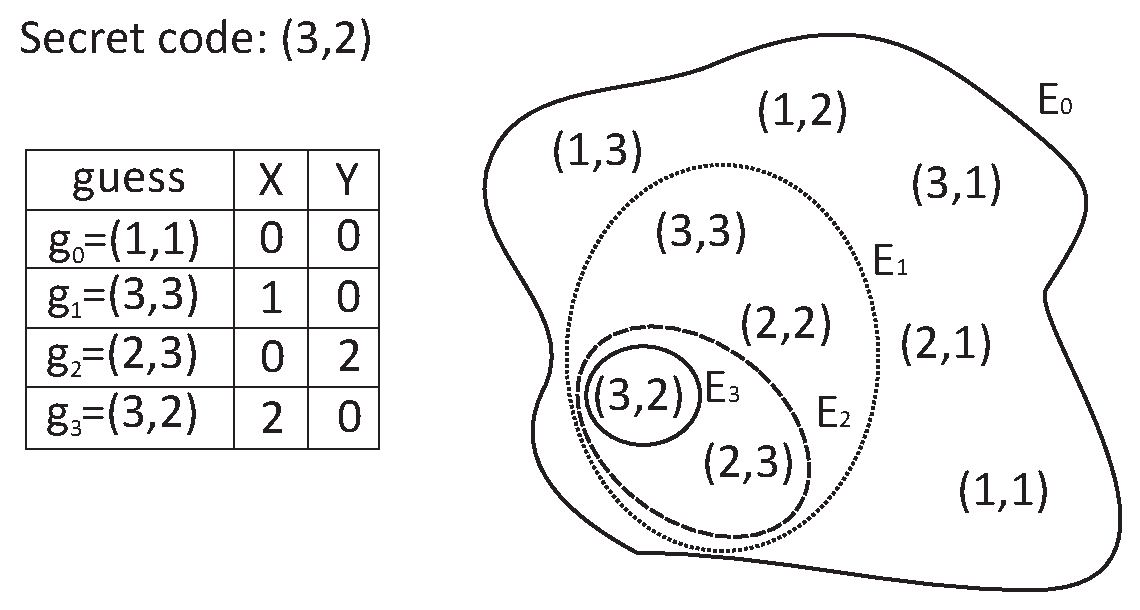
\includegraphics[draft=false,angle=0,width=8cm]{./Particiones_En.eps}
\end{center}
\caption{\label{Particiones_En} Example of the eligible set changes after different guesses in the game.}
\end{figure}

\noindent {\bf Definition:} We denote matrix $XY$ for a given guess ${\bf g}_{n+1}$ as the matrix formed by all the cardinals of the eligible subsets partitions $E_{n+1,r_i}$, i.e., $$XY=\{|E_{n+1,r_1}|,|E_{n+1,r_2}|, \ldots, |E_{n+1,r_k}|\},$$ where $k$ is the number of possible answers to ${\bf g}_{n+1}$.\\

\begin{figure}[!ht]
\begin{center}
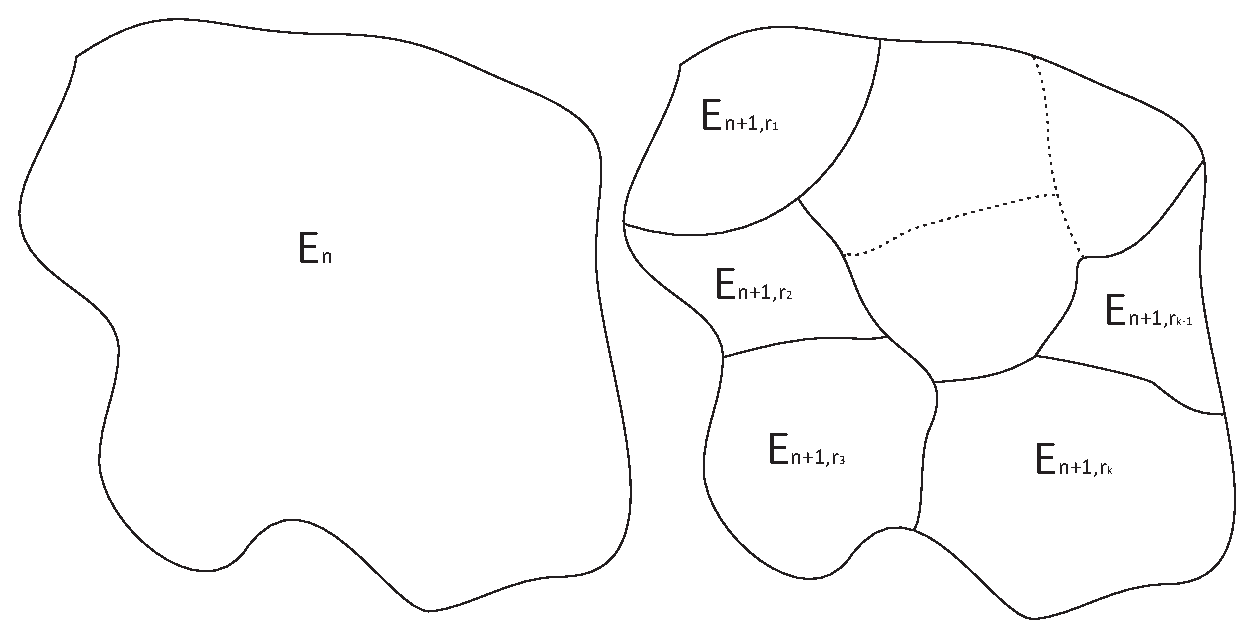
\includegraphics[draft=false,angle=0,width=8cm]{./Particion_XY.eps}
\end{center}
\caption{\label{Partition_XY} Example of eligible subsets partitions once a given guess has been played.}
\end{figure}

\noindent {\bf Definition:} We denote {\em tree game}, $\mathcal{T}_G$ to the tree graph generated by all possible games given a certain strategy.\\

For example, consider the case of $G(2,3)$ games. Figure \ref{TreeGame25} shows an example of $\mathcal{T}_G$ for $G(2,3)$, for the strategy of starting with the guess 11. Note that $\mathcal{T}_G$ shows all possible games starting in ${\bf g}_1=11$.\\

\begin{figure}[!ht]
\begin{center}
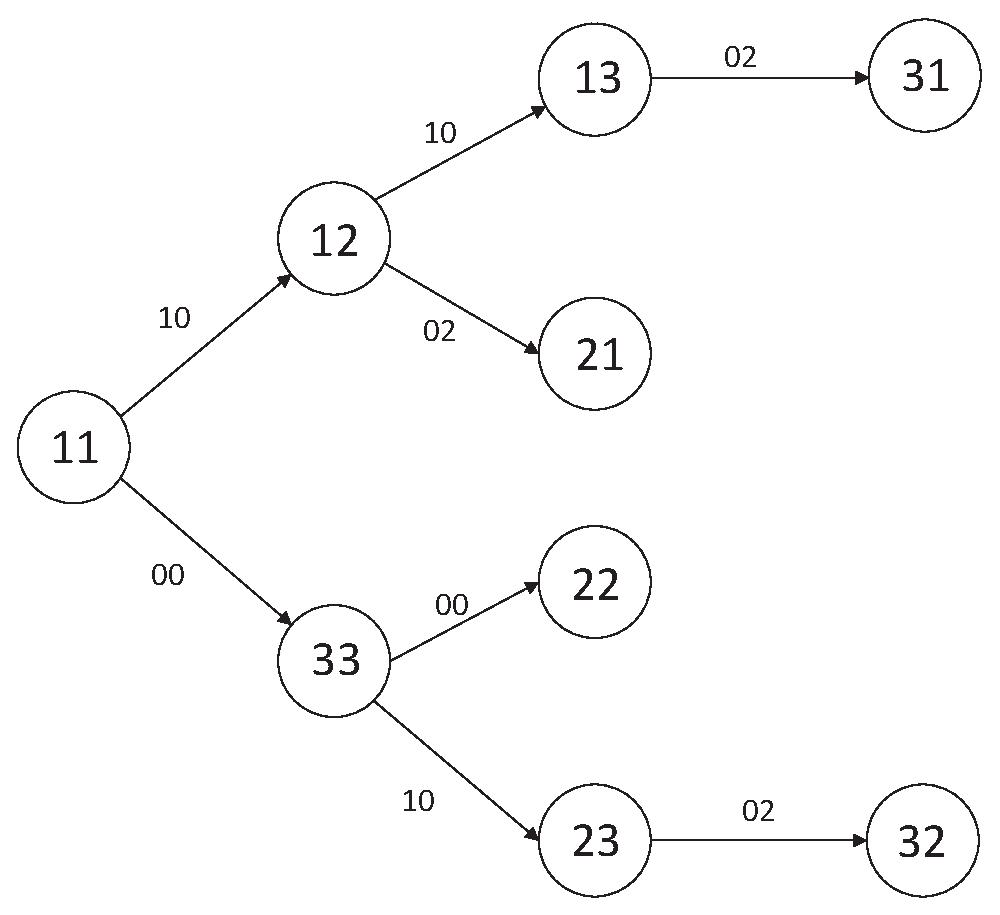
\includegraphics[draft=false,angle=0,width=6cm]{./arbol_peso25.eps}
\end{center}
\caption{\label{TreeGame25} Example of tree game in $G(2,3)$. Numbers in nodes represent guesses (there are 3 colors, 1,2,3), and numbers in links represent answers $X$, $Y$.}
\end{figure}

\noindent {\bf Definition:} We denote {\em tree weight}, $\mathcal{W}(\mathcal{T}_G)$, to the total number of guesses that leads to solve all possible games for a given strategy (tree game).\\

Mathematically this can be expressed in the following way:

\begin{equation}
 \mathcal{W}(\mathcal{T}_G)=\sum_{i=1}^{md} d_i \cdot i
\end{equation}
where $d_i$ stands for the number of nodes of depth $i$ in the tree game, and $md$ stands for the maximum depth of the considered tree game.

As an example, in the tree game of Figure \ref{TreeGame25}, the maximum depth is $md=4$, and $d_1=1$, $d_2=2$, $d_3=4$ and $d_4=2$. The tree weight associated with this tree game is therefore $\mathcal{W}(\mathcal{T}_G)=25$. Note that the tree weight completely depends on the starting strategy chosen for a given MasterMind game. For example, Figure \ref{TreeGame21} shows a different tree game for $G(2,3)$, in this case with minimum tree weight ($\mathcal{W}(\mathcal{T}_G)=21$). Some of the strategies considered later on in the paper for solving the MasterMind are based on minimization of the tree weight for a given game. Finally, note that, given a tree game, the average number of tries to solve the game can be calculated by dividing its weight by the total number of eligible combinations.

\begin{figure}[!ht]
\begin{center}
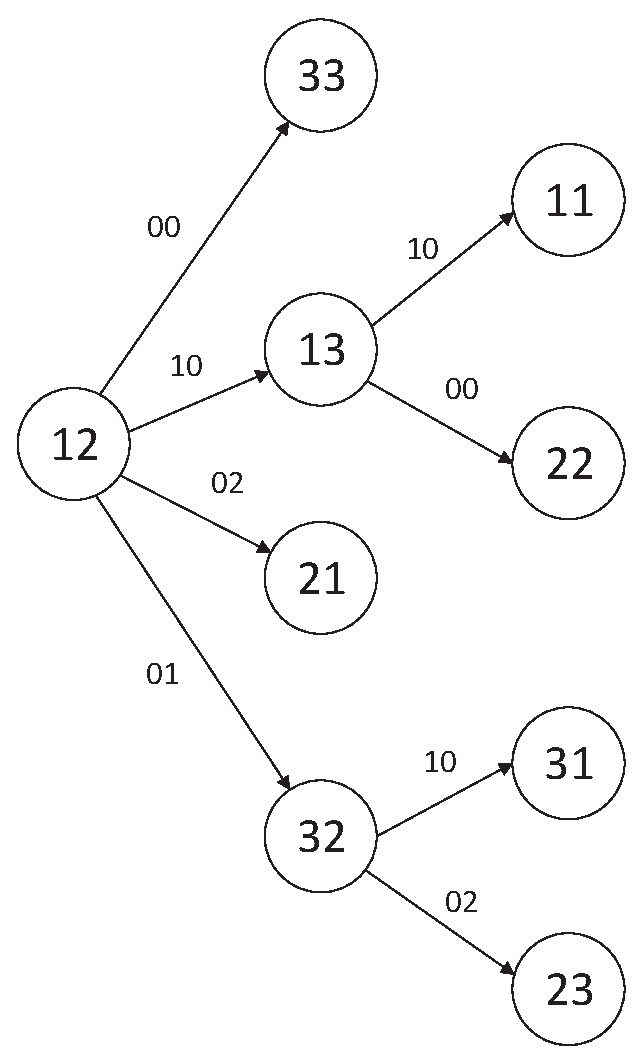
\includegraphics[draft=false,angle=0,width=4cm]{./arbol_peso21.eps}
\end{center}
\caption{\label{TreeGame21} Example of the tree game with minimum tree weight in $G(2,3)$.}
\end{figure}


\section{Proposed nested hierarchical evolutionary approach}
\label{ss:bs}

This section presents the new algorithms proposed in this paper to solve the MasterMind: a Nested Hierarchical Evolutionary Algorithm (NHEA).
The proposed NHEA approach is based on a significant modification of the
evolutionary approach in \cite{Berghman09}. In this case, the selection of the combination played (guess ${\bf g_{n+1}}$)
is obtained by a second evolutionary algorithm, launched for the eligible set $E_n$
from the first evolutionary approach. The final algorithm is therefore a combination of two (nested and hierarchical) evolutionary algorithms,
the first one (Search EA) focused on obtaining the best possible eligible set, and the second one (Decision EA) on providing the optimal guess ${\bf g_{n+1}}$
among the elements in $E_n$. Both algorithms must be run several times to obtain a final solution to the MasterMind. Note that the best individual in the Decision EA provides the information necessary to calculate the fitness for another run of the Search EA.

The Search EA can be described as follows:
For a generic MasterMind game $G(P,N)$, and a first played guess $g_1$, a first initial population is randomly generated containing the different tempted solutions (codes) to the problem. The Search EA aims to obtain a set of codes belonging to the eligible set $E_n$, taking into account the sequence of $n$ previously played codes ($n=1$ in the first generation of the algorithm). The fitness value of each code is calculated by using the expression proposed in \cite{Berghman09}:

\begin{equation}
f({\bf C})=\sum_{i=1}^n 2 \cdot P-|X'_i-X_i|-|Y'_i-Y_i|,
\label{eq:dist}
\end{equation}
where ${\bf C}$ stands for the code to be evaluated, $n$ is the number of codes previously evaluated, $X$, $Y$ are the responses of the code evaluated with respect to the real secret code, and $X'$, $Y'$ stand for the responses give if we consider $C$ as the secret code. Note that when $X'_i$ and $Y'_i$ are equal to $X_i$ and $Y_i$, the value of $f({\bf C})=2 \cdot P \cdot n$, and $C$ belongs to the eligible set $E_n$.

The evolutionary operators applied in this Search EA are one and two points crossover (selected with a probability of 0.5 at the time of their application), and direct random, swapping and inversion mutations (these applied with a small probability). In addition, an operator of hyper-mutation, similar to the one introduced in \cite{Merelo06} is considered after a number of generations. Hyper-mutation consists of re-starting a high percentage of the population to random individuals if some conditions are fulfilled. The selection procedure to choose the parents is the roulette wheel, and a mechanism of elitist population replacement between the initial and the new generated one (after the application of the evolutionary operators) is considered. To do this, the initial and new population are merged together, a percentage of the best individuals are kept, and the rest of the population is completed by randomly choosing the remaining individuals. A diversity mechanism is also applied, in such a way that if two elements in the population are equal, one of them is removed and replaced by a randomly generated individual.

Note that we have set upper and lower bounds for the eligible set size. At the beginning of the algorithm, this size can be huge, whereas in the final steps of the algorithm the eligible set size will be much smaller. In this latter case, the Search EA is stopped when a maximum number of generations have been reached, if there is at least one element in the eligible set.

Once the Search EA has finished its run $n$, an eligible set outcome $E_n$ is obtained. The Decision EA is launched at this stage, in order to come up with the best guess $g_{n+1}$, out of the elements of $E_n$. This process uses specific strategies applied over the eligible set $E_n$ in order to estimate the predictive power of each code in $E_n$. These strategies are the one-step anticipation strategies, i.e. {\em Expected Size} (ES), {\em Most-Parts} (MP), {\em Entropy} (EN) and {\em Worst Case} (WC). The Decision EA uses the same encoding that the Search EA, so we have considered similar operators in both algorithms. The fitness function used depends on the anticipation strategy considered. Note that anticipation strategies determine the prediction power for a combination by means of operations in the $XY$ matrix of the game. Recall that, for a specific point of a game $G(P,N)$, $XY$ represents the way in which a given guess divides the eligible set $E_n$. Let $M$ be the $XY$ matrix of an specific guess $g$, the fitness functions defined for each anticipation strategy are the following:

\begin{equation}\label{ES}
f(M)_{ES}=\sum_{i=1}^k \frac{|E_n|}{|E_{n+1,r_i}|^2},
\end{equation}

\begin{equation}\label{MP}
f(M)_{MP}=\sum_{i=1}^k 1,
\end{equation}

\begin{equation}\label{EN}
f(M)_{EN}=\sum_{i=1}^k -\frac{|E_{n+1,r_i}|}{|E_n|} \cdot \log\left(\frac{|E_{n+1,r_i}|}{|E_n|}\right),
\end{equation}

\begin{equation}\label{WC}
f(M)_{WP}=\frac{|E_n|}{\max(|E_{n+1,r_1}|,|E_{n+1,r_2}|, \ldots, |E_{n+1,r_k}|)},
\end{equation}

In addition, note that $f(M)=0$ if $|E_n|=|E_{n+1,r_j}|$ for any $j \in {1, \ldots, k}$, and $|E_n| \neq 1$ (those combinations that do not reduce the eligible set size do not have any predictive power).


\section{Development of new game strategies for MasterMind based on Genetic Programming}\label{GP}

This section describes the application of Genetic Programming (GP) to the design of novel anticipation strategies for the MasterMind game.
First, some previous important concepts of GP are revised. Then, the GP algorithm specific for the MasterMind is developed.

\subsection{Genetic Programming}

Genetic programming (GP) is one of the methods in the broad field of Genetic and Evolutionary Computation. GP is able to \emph{automatically} create a computer program which solves a complex problem by using the evolution paradigm and the survival of the fittest concept. The research in the area of Genetic Programming (GP) took off in the early 1990's, mainly driven by the key publication of J.R. Koza \cite{Koza92a}. Today, there are dozens of excellent books on GP and its numerous and varied applications \cite{Koza92b}-\cite{Angeline96}.

The basic steps that define the way GP works are:

\begin{enumerate}
\item Randomly create an \emph{initial population of programs} from the available \emph{primitives} $-$the set of allowed functions, variables and constants. In order to properly manage the programs, these usually adopt the form of tree graph structures, where functions are in the intermediate nodes, and variables and constants in the leaves nodes. Finally, each program is formed by a tree graph, whose nodes, links and leaves establish the order and relationship between operations in the program. Then, the following loop is carried out to evolve programs:

% Hay un entorno "Algorithm" que podrías usar y tiene mucha mejor
% pinta - JJ
\item \textbf{Repeat}

\item Run each program and compute its \emph{fitness} (a numerical measure of how well it solves the problem).

\item \emph{Select}, with a probability based on such fitness, one or two program(s) from the population to participate in genetic operations.

\item Create new candidate program(s) by applying genetic operators with specified probabilities (crossover and mutation operators over the tree graphs).

\item \textbf{until} an suitable solution is found or some other stopping condition is achieved.

\item Return the \emph{best}-so-far \emph{program} for solving the considered problem.

\end{enumerate}

In this case, we show how to apply GP to the obtention of robust new strategies for MasterMind.

\subsection{New MasterMind anticipation strategies with GP}

Strategies in MasterMind are associated with objective functions to determine the predictive power of possible codes. Thus, any try to set new strategies for this game will consist of establishing new objective functions to this end. First, note that existing strategies (ES, MP and EN) could be written in the following form\footnote{We do not consider WC since it is focussed on minimizing the maximum depth of the game tree, instead of minimizing the tree weight. ES, MP and EN are focussed on minimizing the tree weight, and are known to be more efficient than WC.}:

\begin{equation}\label{sum_generico}
f(M)=\sum_{i=1}^k Operators(terminals).
\end{equation}
This point can be checked out by simple inspection of Equations (\ref{ES}) to (\ref{EN}). In fact, this means that these strategies can be written in the form of a graph tree.

\begin{figure}[!ht]
\begin{center}
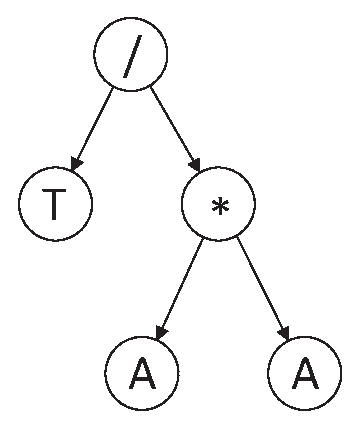
\includegraphics[draft=false,angle=0,width=3cm]{./ES_tree.eps}
\end{center}
\caption{\label{Estrategia_ES} Example of tree encoding of the ES classic strategy for MasterMind..}
\end{figure}

\begin{figure}[!ht]
\begin{center}
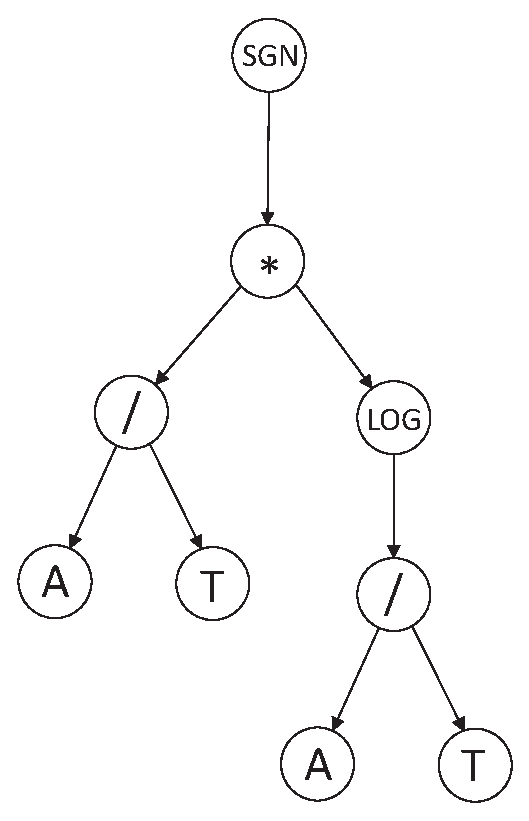
\includegraphics[draft=false,angle=0,width=3cm]{./EN_tree.eps}
\end{center}
\caption{\label{Estrategia_EN} Example of tree encoding of the EN classic strategy for MasterMind.}
\end{figure}

Figures \ref{Estrategia_ES} and \ref{Estrategia_EN} show the tree representation of strategies ES and EN, where $A=|E_{n+1,r_i}|$, $B=1$, $T=|E_n|$, $LOG=\log(x)$ and $SGN$ stands for a change of sign. Following this, we consider the problem of new strategies design as a problem of creating new tree graph structures (optimal with respect to a given objective function), which represent the operations inside the general formula given by Equation (\ref{sum_generico}). This process can be carried out by applying a GP algorithm, with terminals and functions given in Table \ref{tab:GPparams}.

\begin{table}[h!]
\centering
\caption{Functions and terminals used in the GP algorithm for obtaining new MasterMind strategies. \label{tab:GPparams}}
\begin{tabular}{lccc}
\hline
Parameter & Value \\
\hline \\
Functions  & -, +, *, /, $\sqrt{}$, $\log$, SGN\\
Terminals & A, B, C, X, Y, T\\
\hline
\hline
Function & definition\\
\hline
- & substration\\
+ & sum\\
* & multiplication\\
/ & division\\
$\sqrt{}$ & square root\\
$\log$ & natural logarithm\\
SGN & change of sign\\
\hline
\hline
Terminal & definition\\
\hline
A & $|E_{n+1,r_j}|$\\
B & 1 \\
C & number of non-null elements of matrix $XY$\\
X & number of black pegs in response $i$: $X$\\
Y & number of white pegs in response $i$: $Y$\\
T & $|E_{n}|$\\
\hline
\end{tabular}
\end{table}

Each individual in the GP algorithm is a tree graph containing
elements of Table \ref{tab:GPparams}. The population is randomly
generated taking into account a maximum allowed depth. Then
evolutionary operators (crossover and mutation) are applied. Crossover
consists of generating new trees offspring from randomly chosen
couples of existing ones. We have applied the classic crossover for
tree-graph defined by Koza \cite{Koza92b} % Cita missing - JJ
(shown in Figure \ref{Cruce_GP}), where two crossover points are randomly chosen, and parts of the trees are interchanged.

\begin{figure}[!ht]
\begin{center}
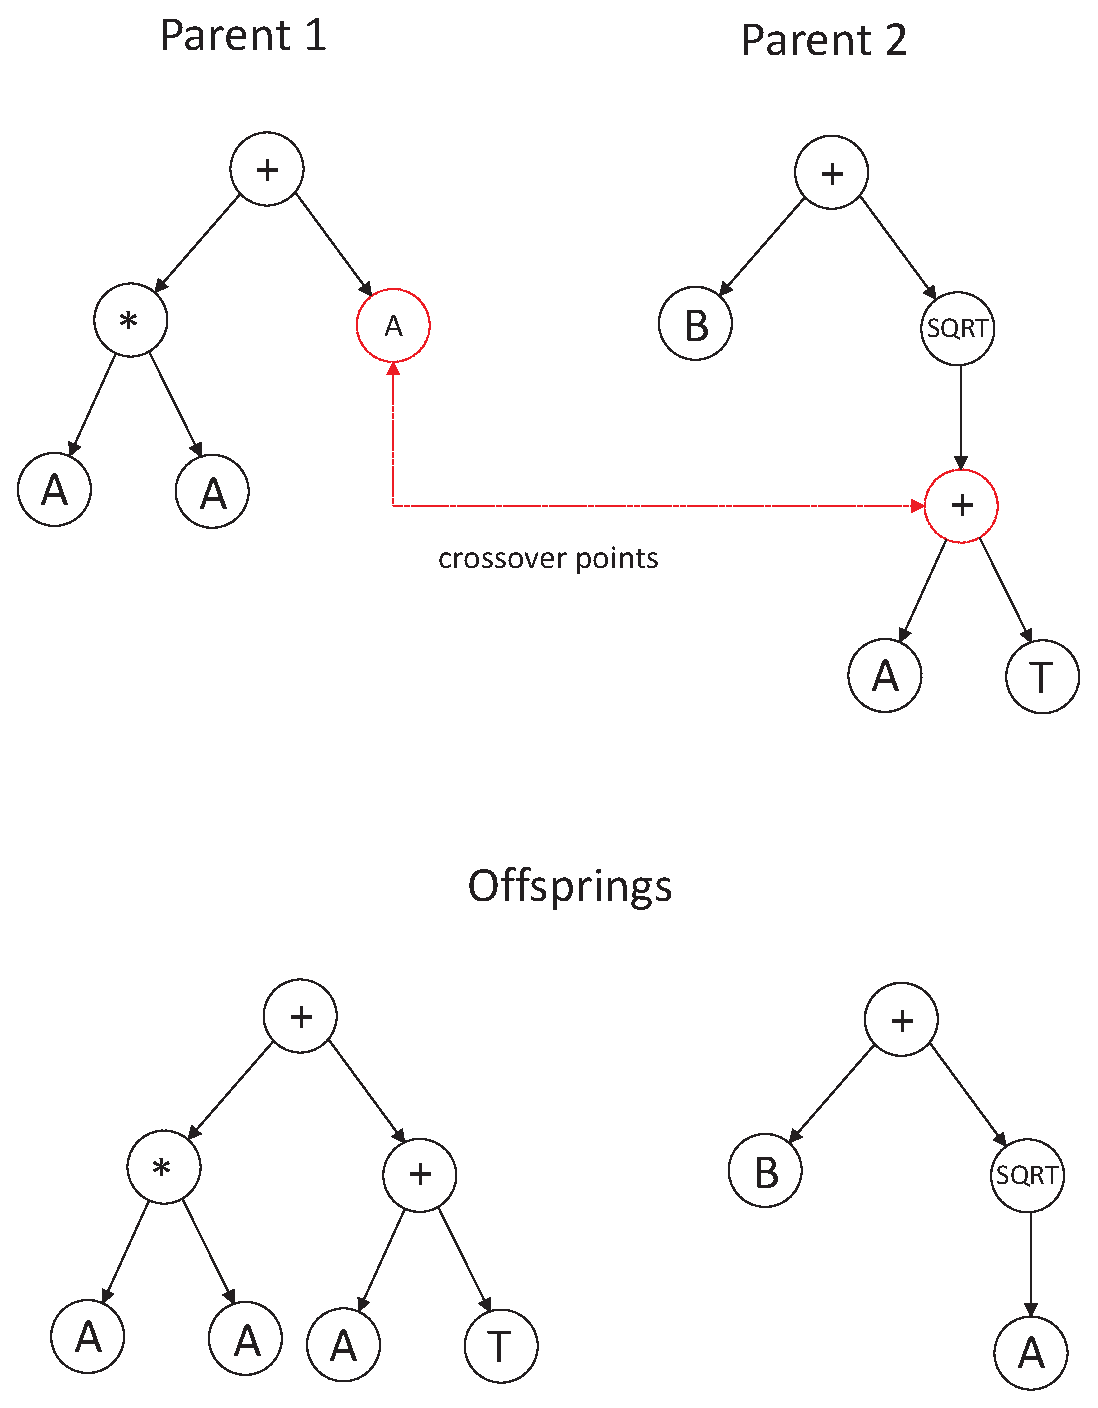
\includegraphics[draft=false,angle=0,width=6cm]{./Cruce_GP.eps}
\end{center}
\caption{\label{Cruce_GP} Example of the classical crossover used in the GP algorithm.}
\end{figure}

We consider four different types of mutations in the GP. First, the classical one, where a piece of a tree is removed and substituted by another one, randomly generated. Figure \ref{classical_mutation_GP} shows an example of this mutation. In this work, we call this procedure as {\em classical tree mutation}. Note that classical mutation is able to change the tree depth. In addition, we define other 3 types of mutations: terminal mutation, functional mutation and mutation by permutation of branches. Figure \ref{mutaciones2} shows an example of these operators. Note that these mutations do not change the tree depth in the algorithm. Finally, a roulette wheel selection is carried out, in order to select the new population for the next generation.

\begin{figure}[!ht]
\begin{center}
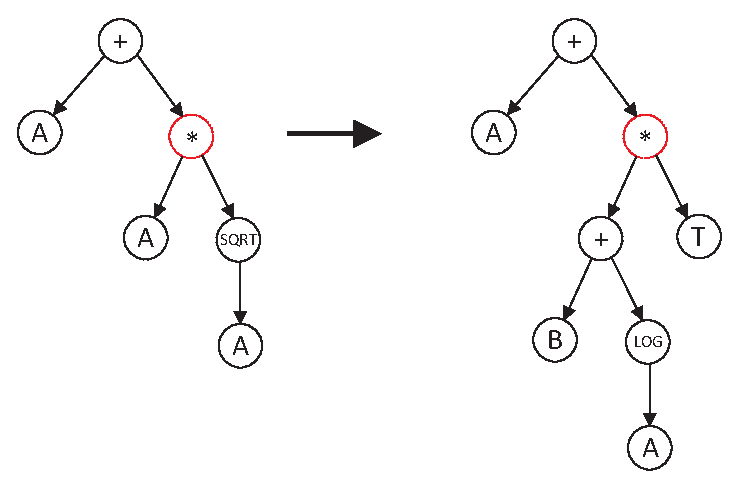
\includegraphics[draft=false,angle=0,width=6cm]{./classical_tree_mutation.eps}
\end{center}
\caption{\label{classical_mutation_GP} Examples of the classical tree mutation in GP.}
\end{figure}

\begin{figure}[!ht]
\begin{center}
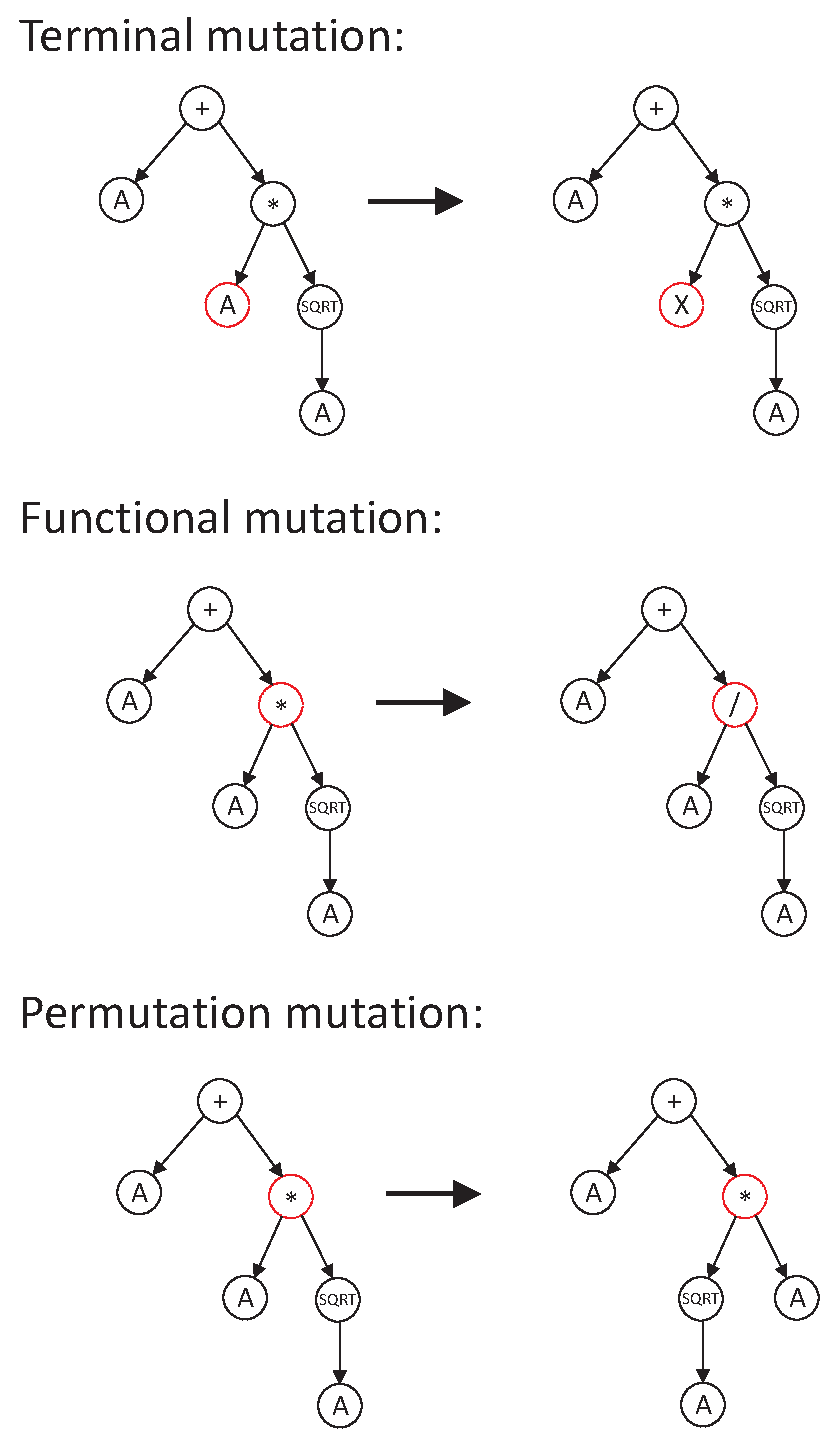
\includegraphics[draft=false,angle=0,width=6cm]{./mutaciones2.eps}
\end{center}
\caption{\label{mutaciones2} Example of terminal mutation, functional mutation and mutation by permutation of branches in GP.}
\end{figure}

Once the population is formed, and the evolutionary operators have been defined, the only missing point to complete the GP algorithm is the fitness function to be maximized. The procedure for obtaining the fitness value of each individual is the following:

\begin{itemize}
\item[1.] Choose a set of $\mathcal{K}$ MasterMind instances $G(P_i,N_i)$, $i=1, 2, \ldots, \mathcal{K}$.
\item[2.] In each instance, obtain the tree games that the current strategy to be evaluated generates, by evaluating in each node the maximum predictive power combinations.
\item[3.] Determine $\mathcal{W}_{max}(\mathcal{T}_{G(P_i,N_i)})$ and $\mathcal{W}_{min}(\mathcal{T}_{G(P_i,N_i)})$ (maximum and minimum weights) of the generated trees for all the considered instances.
\item[4.] Assign a fitness value to the strategy, using the following expression $$f(\mathcal{T}_G)=\frac{1}{\sum_{i=1}^{\mathcal{K}}\left(\mathcal{W}_{min}(\mathcal{T}_{G(P_i,N_i)})+\mathcal{W}_{max}(\mathcal{T}_{G(P_i,N_i)})\right)}$$
Note that this fitness function returns high values for strategies that generate tress with reduced weight, within a reduced margin (difference between the maximum and minimum weights of the trees). Note also that, given a specific anticipation strategy, the game must be played with a search algorithm, and the quality of the strategy is associated with the search algorithm used in this phase. In this case, we use an evolutionary algorithm similar to the one presented in Section \ref{ss:bs}, that implements a width-search (instead of a heuristic search) over the total of the elements in the eligible set.
\end{itemize}

\section{Experimental results}\label{Experiments}

\subsection{Stepwise evolutionary approach for comparison}
\label{ss:evo}

For comparison purposes with the solver presented in this work, we use a previously discussed approach introduced in \cite{Merelo06}, and called {\em evo++} hereafter. It uses a single evolutionary algorithm to first find feasible
solutions and then continue evolution for a few generations within the
set of feasible solutions so that there is a certain degree of
optimization of the score of feasible solutions. In that sense, it is
also similar to Berghman's although the way of obtaining the score is
completely different.

The fitness function used by this method combines the two evolutionary algorithms
mentioned above in a single one. First factor is the {\em distance to
  feasibility} used by the Search EA above. Instead of Equation (\ref{eq:dist}),
this formula is used:
\begin{equation}
f({\bf C})=\sum_{i=1}^n |X'_i-X_i|-|Y'_i-Y_i|,
\label{eq:dist2}
\end{equation}
Unlike above, $C$ is eligible when f({\bf C}) is 0.
In that case, the second factor is considered. This second factor
includes the feasibility score, but instead of using the expected
value as in the Decision EA above (expressed in Equation (\ref{ES}) and
subsequent), two different scoring methods are used: Entropy (called
EN above) and Most Parts (MP). These two factors (which we can call
``search'' and ``decision'' terms, $f_S$ and $f_D$ are then combined
in a single fitness function as follows:
\[
f({\bf C}) = f_D(C) + 1-\min_k \{f_S(k)\}
\]
where $k$ runs over all non-feasible combinations in the
population. This implies that the worst non-feasible combination will
have fitness equal to 0, and all feasible combinations have a fitness
that is above all non-feasible combinations.

This evolutionary algorithm has been also optimized so that the
maximum number of evaluations achieved in the worst case is
minimized. The only change with respect to results already published
is that, besides using the MP strategy, we have used here for the
first time EN. Results will be shown in the next section.

\subsection{Performance of the nested hierarchical evolutionary approach}

The experiments were done just on two problem instances, $G(5,8)$ and $G(6,9)$. These are difficult enough to be able
to make the quality of the different algorithms apart, but also simple
enough to perform the experiments in an amount of time that is
affordable. The experiments were performed on a published set of 5000
instances and playing a single game for each instance. Experiments
for NHEA and Evo++ were done on different computers. Evo++ used a single
parametrization, shown in table \ref{tab:params} except for population
and consistent set size. Population and consistent set size are found
by testing different values and using rules of thumb (consistent set
size should be approximately 1/10 of the population size). However, the
results in this case are not guaranteed to be the best; we stopped
when we found the best average number of moves, but from that point
population and consistent set size (and thus number of evaluations)
could be improved.

\begin{table}[!ht]
\centering
\caption{Values for the Evo++ parameters that obtain the best
  result. Permutation, crossover and mutation are {\em priorities};
  they are normalized to one to convert them to application rates. In
  practice, crossover will be applied to 80\% and mutation and
  permutation to 10\% of the newly generated combinations each. \label{tab:params}}
\begin{tabular}{lc}
\hline
Parameter & Value \\
\hline
Crossover  & 8 \\
Mutation  & 1 \\
Permutation  & 1 \\
Replacement rate  & 0.75 \\
Tournament size & 7 \\
\hline
\end{tabular}
\end{table}
%

Parameters for the NHEA approach are shown in Table \ref{tab:paramsBS}. These parameters are the same for the
Search and Decision EAs in the NHEA algorithm. The specific values of
these parameters were found through systematic experimentation


\begin{table}[!ht]
\centering
\caption{Values for the NHEA parameters used in the simulations. \label{tab:paramsBS}}
\begin{tabular}{lc}
\hline
Parameter & Value \\
\hline
One point Crossover Prob.  & 0.5 \\
Two points Crossover Prob. & 0.5 \\
Mutation  & 0.03 \\
Inversion  & 0.02 \\
Swapping & 0.03 \\
\hline
\end{tabular}
\end{table}

Two different measures of quality were used: the average
number of moves and the number of evaluations. The first is a measure
of the quality of the algorithm playing the game, and the second of
algorithm performance; being EAs search algorithms, the smaller
percentage of the search space that is explored, the better. Results
are shown in Table \ref{tab:comparison-guesses}.


\begin{table*}[!ht]
\centering
\caption{Comparison among approaches in this paper: NHEA, Evo++
  and Berghman et al. \cite{Berghman09}. \label{tab:comparison-guesses}}
\subfigure[Mean number of guesses with standard deviation;
the quantities in parentheses indicate population and consistent set
size (in the case of Evo++). The horizontal line
indicates significant differences using Wilcoxon paired test. There
is also significant difference for  $G(6,9)$ between the two
versions of Evo++, but not in the other case.\label{tab:moves}]{
% Era 80 el tamaño de conjunto consistente que se usaba? Siempre es el
% mismo? No se dice en ningún lado - JJ
\begin{tabular}{lcc}
\hline
                    &$G(5,8)$ & $G(6,9)$ \\
\hline
Berghman et al. &                                           & 6.475  \\
\textsc{Evo++ (EN) }   & (1000,200) $ 5.555 \pm 0.011$ & (2000,200)
$6.373 \pm 0.011$ \\
\textsc{NHEA}  & $5.518 \pm  0.009$ &  $6.382 \pm 0.011 $ \\
\hline
\textsc{Evo++ (MP) }   & (1000,80) $ 5.602 \pm 0.012$ & (2000,200)
$6.436 \pm 0.012$ \\

\hline
\end{tabular}
}

\subfigure[Mean number of evaluations with standard deviation;
differences are always significant.\label{tab:evals}]{
\begin{tabular}{lcc}
\hline
                    &$G(5,8)$ & $G(6,9)$ \\
\hline
\textsc{Evo++ (EN) }   &  $ 26098 \pm 144$ & $67521 \pm 384$ \\
\textsc{NHEA}  & $40619 \pm  115 $ &  $45478 \pm 168 $ \\
\textsc{Evo++ (MP) }   & $20120 \pm 114$ & $68860 \pm 406$ \\

\hline
\end{tabular}
}
\end{table*}

The first outstanding result, looking at Table \ref{tab:moves} is that
NHEA and Evo++ are able to obtain roughly the same results
(statistically insignificant difference) using Entropy as score, even
if the methods to obtain the consistent set, and even the size of the
set, is completely different; at the same time, we can say that it is
also proved that EN is significantly better than MP at least for these
sizes, even if at smaller sizes there is not a significant difference,
at least in exhaustive search studies \cite{Merelo12}. We could thus
affirm that the main factor in optimizing the number of moves is the
scoring method.

The conclusion is not so clear regarding the evaluations, and thus the
running time that depends on it. These are shown in Table
\ref{tab:evals}. Evo++ in all versions beats NHEA for the smaller
size. However, its results are much worse for the bigger size
$G(6,9)$. In that sense, and taking into account both
results, we could say that depending on the size, NHEA or Evo++ (EN) are
the best methods. Evo++ (MP) is always dominated, in both senses, by
the other methods. This supports the conclusion, advanced in the
abstract, that Entropy is a better scoring strategy than Most Parts;
both were proved better than the rest (at least for small sizes) in
\cite{Runarsson10}, which leads us to conclude that, to minimize the
number of moves needed to obtain the solution, Entropy should be used, as classical strategy,
to score eligible solutions.

\subsection{Evaluation of the GP for MasterMind strategies generation}

This section describes the performance of the proposed GP algorithm in the generation of MasterMind anticipation strategies. The methodology carried out has been the following: the proposed GP algorithm described in Section \ref{GP} has been applied to generate new strategies, by choosing $\mathcal{K}=6$ specific MasterMind games to run the algorithm (a kind of ``training set of problems''). The strategies are evaluated over eligible sets, and the main parameters of the GP are given in Table \ref{tab:paramsGP}. The specific 6 problems to train the strategies are $G(4,6)$, $G(7,3)$, $G(4,7)$, $G(5,5)$, $G(4,8)$ and $G(6,4)$. On the other hand, after obtaining the optimal strategies, these have been tested in alternative problems, comparing their performance with that of classical strategies. The problems to test the strategies obtained are $G(4,9)$, $G(5,7)$, $G(6,5)$, $G(7,4)$ and $G(8,3)$.

\begin{table}[!ht]
\centering
\caption{Parameters of the proposed GP in the simulations carried out to establish its performance. \label{tab:paramsGP}}
\begin{tabular}{lc}
\hline
Parameter & Value \\
\hline
Population & 40\\
Generations & 300\\
Crossover Prob.  & 0.9 \\
Functional mutation Prob. & 0.1 \\
Terminal mutation Prob. & 0.2\\
Tree mutation Prob. & 0.2\\
Permutation mutation Prob. & 0.2\\
\hline
\end{tabular}
\end{table}

Table \ref{Nuevas_estrategias} shows the best 5 strategies obtained
with the GP algorithm. We have named them as M1 to M5 strategies. They
are encoded using the terminals defined in Table
\ref{tab:GPparams}. In order to evaluate the quality of the obtained
strategies, Table \ref{Resultados_estrategias} shows the minimum and
maximum weights obtained with them, in comparison with the results
obtained with the classical strategies ES and EN. It is easy to see
that the prediction power of the new strategies generated is equal or
better than the classical ones. For all the games analyzed, at least
one strategy M1 to M5 reduces the minimum weight of the tree game, and
in addition, the obtained weight margin (difference between the
minimum and maximum tree weights) is small in all the new
strategies. This shows that these strategies, obtained with the
proposed GP approach,  are better than the classical ones for the MasterMind game, so they will obtain better results when applied within a search algorithm.


\begin{table}[!ht]
\centering
\caption{Best MasterMind anticipation strategies obtained with the GP algorithm. \label{Nuevas_estrategias}}
\begin{tabular}{lc}
\hline
Strategy & Expression\\
\hline \\
M1& $T-A^2$\\
M2& $(4-A) \cdot \sqrt{A+2}$\\
M3& $(A+1) \cot C + \sqrt{T-\frac{A}{C}}$\\
M4& $\log(A) \cdot (A \dot (\sqrt{A}-1)+\sqrt{C})\cdot \frac{C-T}{C}$\\
M5& $\left(C-\frac{C}{A}\right) \cdot \left(T+\frac{A+1}{C}\right)$\\
\hline
\end{tabular}
\end{table}


\begin{table}[!ht]
\centering
\caption{Results of the new MasterMind strategies in test problems. \label{Resultados_estrategias}}
\begin{tabular}{lcccccccccccccc}
\hline
&\multicolumn{2}{c}{G(4,9)}&\multicolumn{2}{c}{G(5,7)}&\multicolumn{2}{c}{G(6,5)}&\multicolumn{2}{c}{G(7,4)}&\multicolumn{2}{c}{G(8,3)}\\
Strategy         & $\mathcal{W}_{min}$&$\mathcal{W}_{max}$& $\mathcal{W}_{min}$&$\mathcal{W}_{max}$& $\mathcal{W}_{min}$&$\mathcal{W}_{max}$& $\mathcal{W}_{min}$&$\mathcal{W}_{max}$& $\mathcal{W}_{min}$&$\mathcal{W}_{max}$\\
\hline \\
ES&35728&35776&87039&87157&75016&75126&77569&77685&29786&29815\\
EN&35678&35685&87368&87403&74869&74889&77323&77341&29768&29777\\
\hline
\hline
M1&35697&35723&86889&86932&74775&74811&77264&77323&29669&29693\\
M2&35676&35685&87334&87368&74805&74825&77382&77419&29743&29763\\
M3&35725&35734&86942&86969&74866&74893&77178&77211&29162&29192\\
M4&35685&35693&86916&86946&74792&74819&77258&77288&29181&29208\\
M5&35717&35742&86931&86975&74861&74895&77171&77228&29151&29206\\
\hline
\end{tabular}
\end{table}

% Deberías hacer algún tipo de análisis estadístico para probar que
% efectivametne son mejores y en qué grado - JJ

%\begin{table}[h!]
%\centering
%\caption{Results of the new MasterMind strategies in test problems (global). \label{Resultados_estrategias}}
%\begin{tabular}{lcccccccccccccc}
%\hline
%&\multicolumn{2}{c}{G(4,9)}&\multicolumn{2}{c}{G(5,7)}&\multicolumn{2}{c}{G(6,5)}&\multicolumn{2}{c}{G(7,4)}&\multicolumn{2}{c}{G(8,3)}\\
%Strategy         & $\mathcal{W}_{min}$&$\mathcal{W}_{max}$& $\mathcal{W}_{min}$&$\mathcal{W}_{max}$& $\mathcal{W}_{min}$&$\mathcal{W}_{max}$& $\mathcal{W}_{min}$&$\mathcal{W}_{max}$& $\mathcal{W}_{min}$&$\mathcal{W}_{max}$\\
%\hline \\
%ES&34807&37179&86113&88181&74320&75986&76412&78761&28641&30035\\
%EN&34784&36840&86134&87732&74273&75670&76284&78344&28588&29890\\
%MP&35005&37571&86604&88641&74454&75941&76629&78494&28604&29877\\
%\hline
%M1&34790&37021&86084&87678&74222&75551&76211&78052&28567&29709\\
%M2&34775&36944&86049&87689&74211&75611&76298&78631&28580&29860\\
%M3&34869&37035&86088&87834&74304&75648&76181&77945&28565&29665\\
%M4&34808&36920&86072&87674&74294&75623&76197&78018&28582&29735\\
%M5&34869&37040&86086&87803&74306&75654&76183&77944&28567&29666\\
%\hline
%\end{tabular}
%\end{table}


\section{Conclusions and future work}\label{Conclusions}

This paper presents two evolutionary approaches to tackle the MasterMind game, in different ways: first
we propose a novel evolutionary search algorithm to solve the game. This novel approach is
a hierarchical algorithm that involves two different evolutionary approaches,
one for selecting the best eligible set and another one to select the best playable
code. We have detailed this new algorithm and carried out an experimental
comparison with two existing evolutionary approaches to draw some interesting
conclusions on the performance of the evolutionary techniques for the
MasterMind. Second, we present a Genetic Programming algorithm that searches for
new anticipation strategies for the game. We have described the approach and
operators used in the GP, and we have tested the method in obtaining new anticipation
strategies for the game, in different instances. These new strategies have been also
tested in comparison with the classical ones in alternative larger MasterMind instances,
with excellent results. 

This work opens new lines of research, both in solvers and game strategies development.
Regarding the solvers, we will try to examine more closely what are
the precise mechanisms that make the algorithms behave differently
with respect to the number of evaluations needed to find a playable
move. In terms of new strategies, we will explore the application of new GP approaches
with different terminals and functions that can lead to better strategies for MasterMind and related games.



 \section*{Acknowledgement}

This work has been partially supported by Spanish Ministry of Science
and Innovation, under project numbers ECO2010-22065-C03-02,
TIN2011-28627-C04-02 and P08-TIC-03903 awarded by the Andalusian
Regional Government, as well as project \#83 from CEI-BioTIC
(http://biotic.ugr.es).


\begin{thebibliography}{1}

\bibitem{Knuth77}
E. Knuth, ``The computer as Master Mind,'' {\em Journal of Recreational Mathematics}, vol. 9, pp. 1-6, 1977.

\bibitem{Irving79}
W. Irving, ``Towards an optimum Mastermind strategy,'' {\em Journal of Recreational Mathematics}, vol. 11, no. 2, pp. 81-87, 1979.

\bibitem{Koyoma93}
K. Koyama and T. Lai, ``An optimal Mastermind strategy,'' {\em Journal of Recrational Mathematics}, vol. 25, no. 4, pp. 251-256, 1993.

\bibitem{Bestavros86}
A. Bestavros and A. Belal, ``Master Mind: a game of diagnosis strategies,'' {\em Bulletin of the faculty of engineering}, Alexandria University, Alexandria, Egypt, 1986.

\bibitem{Kooi05}
B. Kooi, ``Yet another mastermind strategy,'' {\em ICGA Journal}, vol. 28, no. 1, pp. 13-20, 2005.

\bibitem{Chen07}
S. T. Chen, S. S. Lin and L. T. Huang, ``A two-phase optimization algorithm for Mastermind,'' {\em The Computer Journal}, vol. 50, no. 4, pp. 435-443, 2007.

\bibitem{Chen07b}
S. T. Chen, S. Lin, L. Huang and S. Hsu, ``Strategy optimization for deductive games,'' {\em European Journal of Operational Research}, vol. 183, pp. 757-766, 2007.

\bibitem{Merelo12}
J. J. Merelo, A. M. Mora, C. Cotta, T. P. Runarsson,
``An experimental study of exhaustive solutions for the Mastermind puzzle,''
{\em ARXiV}, 2012.

\bibitem{Shapiro83}
E. Shapiro, ``Playing Mastermind logically,'' {\em SIGART Bulleting}, vol. 85, pp. 28-29, 1983.

\bibitem{Swaszek00}
P. Swaszek, ``The mastermind novice,'' {\em Journal of Recreational Mathematics}, vol. 30, pp. 130-138, 2000.

\bibitem{Kovacs03}
A. Temporal and T. Kovacs, ``A heuristic hill climbing algorithm for Mastermind,'' In {\em Proc. of the UK workshop on Computational Intelligence}, pp. 183-196, Bristol, UK, 2003.

\bibitem{Bernier96}
J. Bernier, C. Herr\'aiz, J. J. Merelo-Guerv\'os, S. Olmeda and A. Prieto, ``Solving Mastermind using GAs and simulated annealing: a case of dynamic constraint optimization,'' In {\em Proc. of the 4th International Conference on Parallel Problem Solving from Nature}, pp. 554-563, London, UK, 1996.

\bibitem{Bento99}
L. Bento, L. Pereira and A. Rosa, ``Mastermind by evolutionary algorithms,'' In {\em Proc. of the sixth annual workshop on selected areas in cryptography}, pp. 307-311, Kingston, Ontario, Canada, 1999.

\bibitem{Kalister03}
T. Kalister and D. Camens, ``Solving Mastermind using genetic algorithms,'' In {\em Proc. of the Genetic and Evolutionary Computation Conference (GECCO)}, pp. 1590-1591, Chicago, USA, 2003.

\bibitem{Merelo06}
J. J. Merelo-Guerv\'os, P. Castillo and V. Rivas, ``Finding a needle in a haystack using hints and evolutionary computation: the case of evolutionary MasterMind,'' {\em Applied Soft Computing}, vol. 6, no. 2, pp. 170-179, 2006.

\bibitem{Maestro13}
J. Maestro-Montojo, J. J. Merelo and S. Salcedo-Sanz,
``Comparing evolutionary algorithms to solve the game of MasterMind,''
{\em Applications of Evolutionary Computation},
Lecture Notes in Computer Science, vol. 7835, pp. 304-313, 2013.   


\bibitem{Berghman09}
L. Bergman, D. Goossens and R. Leus, ``Efficient solutions for Mastermind using genetic algorithms,'' {\em Computers \& Operations Research}, vol. 36, no. 6, pp. 1880-1885, 2009.

\bibitem{Runarsson10}
T. P. Runarsson and J. J. Merelo-Guervos,
``Adapting heuristic Mastermind strategies to evolutionary algorithms,''
{\em Proc. of the International Workshop on Nature Inspired Cooperative Strategies for Optimization}, Granada, Spain, 2010.

%\bibitem{Goddard}
%W. Goddard``Matermind Revisited,'' {\em Journal of Combinatorial Mathematics and Combinatorial Computing}, vol. 51, pp. 215-220, 2004.
%
%\bibitem{Goodrich09}
%M. T. Goodrich, ``On the algorithmic complexity of the Mastermind game with black-peg results,'' {\em Information Processing Letters}, vol. 109, no. 13, pp. 675-678, 2009.

%\bibitem{Doerr12}
%B. Doerr, R. Sp\"ohel, H. Thomas and C. Winzen,
%``Playing Mastermind with many colors,'' In {\em Proc. of the 11th Cologne-Twente Workshop on Graphs and Combinatorial Optimization}, Munich, Germany, 2012.

%\bibitem{Viglietta12}
%G. Viglietta, ``Hardness of Mastermind,'' In {\em Sixth International Conference on Fun with Algorithms}, 2012.

\bibitem{Koza92a}
J.R. Koza, ``Genetic Programming: On the Programming of Computers by Means of Natural Selection'', MIT Press, Cambridge, MA, USA, 1992.

\bibitem{Koza92b}
J.R. Koza, ``Genetic Programming'', 1992

%\bibitem{Koza94a}
%J.R. Koza, ``Genetic Programming II: Automatic Discovery of Reusable Programs'', 1994
%
%\bibitem{Koza99}
%J.R. Koza, ``Genetic Programming 3'', 1999.
%
%\bibitem{Koza03}
%J.R. Koza, ``Genetic Programming 4'', 2003.

\bibitem{Langdon98}
W. B. Langdon, {\em Genetic Programming and Data Structures}, Kluwer, Boston, 1998.

\bibitem{Koza03}
J. R. Koza and R. Poli, ``A Genetic Programming tutorial,'' In {\em Introductory tutorials in optimization, search and
decision support}, Chapter 8, E. Burke Editor, 2003.

\bibitem{Koza10}
J.R. Koza, ``Human-competitive results produced by genetic programming,'' \emph{Genetic Programming and Evolvable Machines}, vol. 11, pp. 251--284, 2010.

\bibitem{Angeline96}
 {\em Advances in Genetic Programming 2}, P. J. Angeline and K. E. Kinnear Jr., editors, MIT Press, Cambridge, MA, USA, 1996.




\end{thebibliography}




\end{document}
